% Created: Enze Chen, June 2017
% Last edited: Enze Chen, December 2017
%
% Chapter 2 of the MSE 142 coursereader. This chapter develops the time-dependent and time-independent Schrodinger equations. The focus is less on the math and more on the analysis of the wave function solutions, such as Born's statistical interpretation, the normalization condition, and the superposition principle.

% Uncomment the following three lines and last line to individually compile this chapter
%\documentclass[12pt, english]{book}
%\usepackage{142crstyle}
%\begin{document}

\chapter{The \Sch\ Equation} \label{ch:sch}
%{ \doublespacing 
We ended the previous chapter with Louis de Broglie's landmark hypothesis that all matter can behave as both particles and waves. If the de Broglie hypothesis was true, then we would expect there to be a function that can describe the wave amplitude of these particles. We will loosely derive this function and analyze it closely in this chapter, as it is central to quantum mechanics and everything we do in this course. \par 

\section{Introduction to waves}
Recall that in 1924, Louis de Broglie derived the following relations:
\begin{tcolorbox}[title=de Broglie relations] \vspace{-2ex}
	\begin{equation*}
		E=\hbar\omega, \qquad p = \hbar k = \frac{h}{\lambda}
	\end{equation*}
\end{tcolorbox}
The following year, Austrian physicist Erwin \Sch\ decided to follow up on this idea and derive an equation that could model the wave-like behavior of particles.\footnote{A copy of the original paper can be found at E. \Sch, \href{https://journals.aps.org/pr/abstract/10.1103/PhysRev.28.1049}{\emph{Phys. Rev.}} \textbf{28}, 1049 (1926).} In classical mechanics, everyone knew that Newton's Second law ($F=ma$) could be solved to derive the position and velocity of any particle at any given time, provided a set of initial conditions. In quantum mechanics, they wished to answer an analogous question: Is there a governing equation that can be solved to describe the time-evolution of a quantum mechanical state given a set of initial conditions? \par 

To work our way up to the final answer, let's first assume that there exists a function for the wave amplitude denoted by $\Psi$ (upper-case ``psi''). We can first express this function as a propagating wave, which is given by
\begin{equation}
	\Psi(x,t) = Ae^{i(kx-\omega t)} \label{eq:propwave}
\end{equation}
where $A$ is the amplitude coefficient (described more in  Section~\ref{sec:normse}), $k$ is the wavenumber, $\omega$ is the angular frequency, and $i$ is the imaginary constant. Even though we won't formally derive Equation~\ref{eq:propwave}, let's take some time to dissect it because it contains a lot of information. We're saying that the function describing wave-like behavior, $\Psi$, is a \textbf{complex exponential} function dependent on two variables, position $x$ and time $t$. Using Euler's formula (see Section~\ref{sec:math}), we can express complex exponentials in terms of sine and cosine functions:
\begin{equation*}
	\Psi(x,t) = Ae^{i(kx-\omega t)} = A\left(\cos(kx-\omega t) + i\sin(kx-\omega t)\right)
\end{equation*}

Though we will switch between both mathematical forms, the second form conveniently captures the wave motion in the sinusoidal functions. Since our function $\Psi$ depends on $t$, we say that it is a \textbf{traveling wave} that propagates through time, where $k$ and $\omega$ are some characteristic properties of the wave that also make the units cancel out (some physical intuition was provided back in Section~\ref{sec:db-hyp}). \par 

To adapt Equation~\ref{eq:propwave} to the quantum mechanical context, let's rewrite it in terms of $p$ and $E$ to obtain
\begin{equation}
	\Psi(x,t) = Ae^{i(kx-\omega t)} = Ae^{i(\hbar kx - \hbar\omega t)/\hbar}  = Ae^{i(px-Et)/\hbar} \label{eq:qwave}
\end{equation}

We're getting closer! Now let's see what happens if we take a couple derivatives of this equation. Specifically, note that
\begin{equation}
	\pdv{\Psi}{t} = -\frac{iE}{\hbar}\Psi 		\label{eq:qwvdt}
\end{equation}
and
\begin{equation}
	\pdv[2]{\Psi}{x} = -\frac{p^2}{\hbar^2}\Psi \label{eq:qwvdx}
\end{equation}
where $\pdv{t}$ represents taking the \emph{partial} derivative of a quantity with respect to $t$ (reviewed in Section~\ref{sec:diff}). These two equations look pretty similar, so let's see if we can relate the two. We can use some clever manipulations from classical mechanics to obtain 
\begin{equation} 
E = \frac{1}{2}mv^2 = \frac{(mv)^2}{2m} = \frac{p^2}{2m}
\end{equation}

Even though we're at the quantum level, this must still hold true. Next, we will conveniently multiply Equation~\ref{eq:qwvdt} by $i\hbar$ and Equation~\ref{eq:qwvdx} by $-\frac{\hbar^2}{2m}$ to find that
\begin{equation*}
	i\hbar \pdv{\Psi}{t} = E\Psi = \frac{p^2}{2m} \Psi = -\frac{\hbar^2}{2m} \left( -\frac{p^2}{\hbar^2}\Psi \right) = -\frac{\hbar^2}{2m} \pdv[2]{\Psi}{x}
\end{equation*}

Equating the first and last terms above, we get 
\begin{equation}
	i\hbar \pdv{\Psi}{t} = -\frac{\hbar^2}{2m} \pdv[2]{\Psi}{x}
\end{equation}
which is the famous \textbf{\Sch\ equation} for a free particle. For a particle that is moving through a non-zero potential $V(x,t)$, we modify our energy function to be $E = \frac{p^2}{2m} + V$ and obtain in full: 
\begin{tcolorbox}[title=Time-dependent \Sch\ equation] \vspace{-2ex}
\begin{equation}
	i\hbar \pdv{\Psi}{t} = -\frac{\hbar^2}{2m} \pdv[2]{\Psi}{x} + V(x,t)\Psi \label{eq:tdse}
\end{equation}
\end{tcolorbox}

Equation~\ref{eq:tdse} is the one-dimensional, time-dependent \Sch\ equation that describes the time-evolution of a quantum mechanical system's \textbf{wave function}, $\Psi$. For the purposes of this course we will only consider one dimension in space (e.g. $x$ direction only). The \Sch\ equation is a \textbf{linear partial differential equation}, which means it depends on the derivatives of a function with respect to multiple variables, i.e. the first partial derivative of $\Psi$ with respect to time and the second partial derivative of $\Psi$ with respect to position. This equation was enthusiastically accepted by the physics community soon after it was proposed as it enabled new interpretations of quantum theory and had many other profound consequences.\footnote{For a Stanford professor's account of the origins of the \Sch\ equation, check out F. Bloch, \href{http://physicstoday.scitation.org/doi/pdf/10.1063/1.3024633}{\emph{Physics Today}} \textbf{29}, 12 (1976).} For example, if we can solve Equation~\ref{eq:tdse} with some initial condition $\Psi(x,0)$, then we can find $\Psi(x,t)$ for all future time.

%%%%%%%%%%%%%%%%%%%%%%%%%%%%%%%%%%%%%%%%%%%%%%%%%%%%%%%%%%%%%%%%%%%%%%%%%%%%%%%%

\section{Probability distribution} \label{sec:prob}
The \Sch\ equation governs the \emph{behavior} of the wave function $\Psi$, but the number one question all students inevitably ask is: ``What \emph{exactly is} the wave function?'' We know that it is a mathematical representation of a system's quantum state, but this definition is still ambiguous, and the fact that $\Psi$ is a complex function only seems to add to the ambiguity. \par 

The now-standard interpretation of the wave function was originally proposed in 1926 by Max Born, who treated solutions of the \Sch\ equation with a statistical interpretation.\footnote{For his influential work on the interpretation of quantum mechanics and the \Sch\ equation, Max Born was awarded the 1954 Nobel Prize in Physics.} Born interpreted $\Psi$ as the \textbf{probability amplitude} and its absolute square (modulus squared) as a \textbf{probability density function}. In statistics, the probability density function gives the probability of a certain event occurring by the area underneath the density curve. Here, the absolute square of $\Psi$, expressed as $\abs{\Psi(x,t)}^2$, gives the probability density. The actual probability can be computed with an integral as follows:
\begin{tcolorbox}[title=Born's statistical interpretation] \vspace{-2ex}
\begin{equation}
	\int_a^b \abs{\Psi(x,t)}^2 \dd{x} = \mathbb{P}\text{(particle is between $a$ and $b$ at time $t$)} \label{eq:wfprob}
\end{equation}
\end{tcolorbox}

which is also shown below graphically in Figure~\ref{fig:wfprob}.
\begin{figure}[!h]
	\centering
	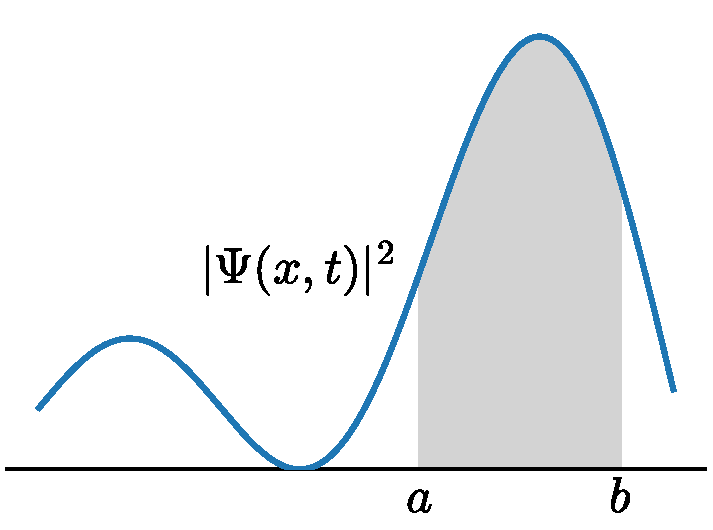
\includegraphics[width=0.4\linewidth]{prob-density}
	\caption{A plot of the absolute square of $\Psi$, with the shaded area representing the probability of finding the particle between points $a$ and $b$.}
	\label{fig:wfprob}
\end{figure}

The statistical interpretation is helpful for many reasons. For one, Equation~\ref{eq:wfprob} helps us reconcile our observations of discrete particles with the continuous nature of the wave function by modeling the latter as a probability. Taking the modulus squared of the wave function also results in a real quantity, since it is equivalent to multiplying the complex wave function by its complex conjugate.
\begin{tcolorbox}[title=Key point: modulus squared of a complex number] \vspace{-2ex}
	\begin{equation}
		\abs{\Psi}^2 = \Psi^*\Psi
	\end{equation}
\end{tcolorbox}

Like any good quantum theory, this interpretation has some strange consequences, the most significant of which is the idea of \textbf{indeterminacy}.\footnote{For a dense read perfect for a Friday evening, check out B. d'Espagnat, \href{https://www.scientificamerican.com/media/pdf/197911_0158.pdf}{\emph{Scientific American}} \textbf{11}, (1979), 158-181.} Notice that we cannot be certain about making measurements of position at the quantum scale, but we can only give a statistical figure as to the \emph{probability} of that result being measured. This is particularly troublesome if a measurement has been made of a particle's position, and then you ask where the particle was \emph{right before} the measurement was made. Was the particle at the same position where you had measured it? If so, why does quantum mechanics still give the possibility, however slight, that it was in fact meters away? And if it wasn't right there, where exactly was the particle?\footnote{\href{http://physicstoday.scitation.org/doi/abs/10.1063/1.880968}{Is the moon there when nobody looks?} N. Mermin, \emph{Physics Today} \textbf{38}, 4 (1985), 38-47.}

%%%%%%%%%%%%%%%%%%%%%%%%%%%%%%%%%%%%%%%%%%%%%%%%%%%%%%%%%%%%%%%%%%%%%%%%%%%%%%%%

\section{Normalization} \label{sec:normse}
However, even when we're surrounded by this uncertainty, there is one thing we \emph{can} be certain of---that \emph{somewhere} in space, the particle must exist and we can find it. This translates mathematically into 
\begin{tcolorbox}[title=Normalization condition] \vspace{-1ex}
	\begin{equation}
	\int_{-\infty}^{+\infty} \abs{\Psi(x,t)}^2 \dd{x} = 1 \label{eq:norm}
	\end{equation}
\end{tcolorbox}

This equation says that the particle is guaranteed to exist in our system at any point in time, which must hold true for the statistical interpretation to make sense. \par 

However, Equation~\ref{eq:norm} also imposes a constraint on the constant factor in the wave function, which we denoted with $A$ back in Equation~\ref{eq:propwave}. Specifically, we have
\begin{align*}
	\int_{-\infty}^{+\infty} \abs{\Psi(x,t)}^2 \dd{x} &= 1 \\
	\int_{-\infty}^{+\infty} \abs{A\Psi(x,t)}^2 \dd{x} &= 1 \\
	\abs{A}^2 \int_{-\infty}^{+\infty} \abs{\Psi(x,t)}^2 \dd{x} &= 1
\end{align*}

This process is called \textbf{normalizing} the wave function. Now we can define $A$ more precisely as a (possibly complex) coefficient that maintains the normalization condition in Equation~\ref{eq:norm}. Amazingly, the \Sch\ equation has the property that it preserves the normalization of the wave function over time, which means that we only have to solve for $A$ once!

%%%%%%%%%%%%%%%%%%%%%%%%%%%%%%%%%%%%%%%%%%%%%%%%%%%%%%%%%%%%%%%%%%%%%%%%%%%%%%%%

\section{Superposition} \label{sec:super}
One of the most important consequences of the \Sch\ equation is that it can correctly model the superposition principle we discussed back in Chapter 1. Recall how we observed in the Stern-Gerlach experiment that the silver atoms seemed to simultaneously exist in two quantum states, $\ket{S^+}$ and $\ket{S^-}$. Could this mean that there exist multiple wave functions that satisfy the \Sch\ equation and collectively describe the behavior of the particle? Absolutely! \par 

Specifically, if we have a wave function $\Psi_1$ that satisfies the \Sch\ equation and a second wave function $\Psi_2$ that also satisfies the \Sch\ equation, then \emph{any linear combination} of the two equations, $\Psi = c_1\Psi_1 + c_2\Psi_2$, is also a valid solution. You might be familiar with this property of linearity if you have already taken a course on differential equations. It allows us to take a set of all possible solutions to the \Sch\ equation and add them together to give a complete representation of all possible quantum states that the particle can be in. \par 

Mathematically, the linearity principle of differential equations provides an explanation for the superposition we previously observed. As improbable as it may have seemed before, we now have yet another reason to believe that particles are capable of simultaneously existing in multiple states. It turns out that we can generalize the result from above even further and decompose any wave function into a sum of distinct quantum states. This is expressed generally as
\begin{tcolorbox}[title=Superposition of wave functions] \vspace{-2ex}
	\begin{equation}
		\Psi = \sum_n c_n\Psi_n  \label{eq:super}
	\end{equation}
\end{tcolorbox}

This equation is the general form that you should keep in mind as we derive more specific instances of the wave function in the following chapters.\footnote{If you have taken a course like CME 104 or MATH 53 here at Stanford, Equation~\ref{eq:super} should seem suspiciously similar to a Fourier series decomposition. While we leave out much of the mathematical hairiness in this course, this is indeed the case, and you can consider the individual wave functions $\Psi_n$ to be eigenstates that form a basis for the space occupied by $\Psi$.}

\section[Time-independence]{Time-independent \Sch\ equation}
Now we will return to the original \Sch\ equation, which was given in Equation~\ref{eq:tdse} as
\begin{equation*}
	i\hbar \pdv{\Psi}{t} = -\frac{\hbar^2}{2m} \pdv[2]{\Psi}{x} + V(x,t)\Psi
\end{equation*}

This is a very complicated differential equation whose general solution is a function of two variables $x$ and $t$. We now consider a special case where the potential function is \emph{time-independent}, i.e. $V=V(x)$, such as that given by a stationary, external electric field. This allows us to apply \textbf{separation of variables} and guess that the solution can be written as a product of two separate functions, each of which is a function of only one variable:\footnote{There's unfortunately no good rationale for why it would occur for us do this, other than ``it's been attempted many times and works well.'' See \href{https://math.stackexchange.com/questions/575205/why-separation-of-variables-works-in-pdes}{math.stackexchange} for a discussion.} 
\begin{tcolorbox}[title = Separation of variables] \vspace{-2ex}
\begin{equation}
	\Psi(x,t) = \psi(x)\phi(t) \label{eq:sep}
\end{equation}
\end{tcolorbox}

Here, $\psi$ (lower-case ``psi'') is a function of $x$ alone, and $\phi$ (lower-case ``phi'') is a function of $t$ alone. This huge simplification allows us to derive a set of interesting solutions that in many cases model quantum mechanical states quite well. Moreover, we've seen in the previous section (Equation~\ref{eq:super}) that it's still possible to superimpose the separable solutions to construct the general solution to the \Sch\ equation. \par

The assumption of time-independent potentials turns the partial differential equation into two ordinary differential equations. We can substitute Equation~\ref{eq:sep} into the \Sch\ equation to obtain
\begin{align*}
	i\hbar \pdv{\Psi}{t} &= -\frac{\hbar^2}{2m} \pdv[2]{\Psi}{x} + V(x,t)\Psi \\
	i\hbar\psi \dv{\phi}{t} &= -\frac{\hbar^2}{2m} \phi\dv[2]{\psi}{x} + V(x)\psi(x)\phi(t) \tag{note the ordinary derivatives now} \\
	i\hbar\frac{1}{\phi} \dv{\phi}{t} &= -\frac{\hbar^2}{2m} \frac{1}{\psi}\dv[2]{\psi}{x} + V(x) \numberthis \label{eq:const}
\end{align*}

Now observe that the left hand side of Equation~\ref{eq:const} is purely a function of $t$ and the right hand side is purely a function of $x$. The only way this equation can be satisfied is if both sides are equal to a \emph{constant} (otherwise, you could vary one side without varying the other by just changing one variable). Let's call this constant $E$, for \textbf{energy}, and we will see why below. In any case, this gives us two equations, one for the left hand side,
\begin{equation}
	i\hbar \dv{\phi}{t} = E\phi \label{eq:phi}
\end{equation}
and another for the right hand side,
\begin{equation}
	-\frac{\hbar^2}{2m} \dv[2]{\psi}{x} + V(x)\psi = E\psi \label{eq:tise}
\end{equation}

Equation~\ref{eq:phi} can be solved using fairly straightforward integration. Specifically, we obtain
\begin{align*}
	i\hbar \dv{\phi}{t} &= E\phi \\
	\int \frac{1}{\phi} \dd{\phi} &= \int -\frac{iE}{\hbar} \dd{t} \\
	\ln \phi &= -\frac{iEt}{\hbar} \\ 
	\Aboxed{\phi(t) &= Ae^{-iEt/\hbar}} \numberthis
\end{align*}
which is another complex exponential function. Equation~\ref{eq:tise}, on the other hand, cannot be solved unless $V(x)$ is specified. In fact, this equation is formally known as the \textbf{time-independent \Sch\ equation} and it can be solved for a variety of simple potentials $V(x)$.
\begin{tcolorbox}[title = Time-independent \Sch\ equation] \vspace{-2ex}
	\begin{equation*}
		-\frac{\hbar^2}{2m} \dv[2]{\psi}{x} + V(x)\psi = E\psi
	\end{equation*}
\end{tcolorbox}

Overall, the solution we have found to Equation~\ref{eq:sep} is
\begin{equation}
	\Psi(x,t) = \psi(x)e^{-iEt/\hbar}
\end{equation}
where we have absorbed the constant $A$ into $\psi(x)$, the solution to the time-independent \Sch\ equation. Here are some further remarks and analyses of the general time-independent solution.
\begin{enumerate}[1.]
	\item The solutions $\psi(x)$ are called \textbf{stationary states} because the probability density is no longer time-dependent. Observe that 
	\begin{equation*}
		\abs{\Psi(x,t)}^2 = \abs{\psi(x)e^{-iEt/\hbar}}^2 = \abs{\psi(x)}^2e^{-iEt/\hbar}e^{iEt/\hbar} = \abs{\psi(x)}^2e^0 = \abs{\psi(x)}^2
	\end{equation*}
	and the time-dependence cancels out. This suggests that nothing is ``occurring'' in a stationary state since the probability of finding a particle does not change with time.
	
	\item Let's go back and address why we labeled the unknown constant as $E$ for energy. Recall that we argued in class that the energy in quantum mechanics could be represented by an \textbf{operator} 
	\begin{equation}
		\hat{E} = i\hbar\pdv{t} \label{eq:Eop}
	\end{equation}
	
	and the momentum by another operator 
	\begin{equation}
		\hat{p} = -i\hbar\pdv{x} \label{eq:Pop}
	\end{equation}
	
	Operators can be considered as special functions that map between different physical states and we distinguish them from their classical values with a hat symbol. Viewed in this way, we see that the time-independent \Sch\ equation is just a statement that the total energy is given by the sum of the kinetic energy and the potential energy. It is reassuring to see that conservation of energy also applies at the quantum level! In fact, this sum is another operator in and of itself, known as the \textbf{Hamiltonian},
	\begin{tcolorbox}[title = Hamiltonian operator] \vspace{-2ex}
		\begin{equation}
		\hat{H} = -\frac{\hbar^2}{2m}\pdv[2]{x}+V(x) \label{eq:ham}
		\end{equation}
	\end{tcolorbox}
	which allows us to write the time-independent \Sch\ equation as
	\begin{equation}
		\hat{H}\psi = E\psi \label{eq:tise-ham}
	\end{equation}
	
	Conveniently, the time-independent \Sch\ equation expressed in this form shows that stationary states have a single \emph{definite energy} that is invariant with respect to time, instead of a superposition of different energies. We will definitely see the Hamiltonian again in later chapters.
	
	\item Last but not least, we note that we have a solution for finding \emph{a particular} solution, but not the general solution. As alluded to in the previous section, we can actually find a set of solutions labeled by an index $n$. Due to the superposition principle, we can construct the general solution to the time-dependent \Sch\ equation\footnote{Note our language here: Superposition states \emph{cannot} be a solution to the time-\emph{independent} \Sch\ equation anymore, as each term would have a different energy value.} as a quantum superposition state given by
	\begin{tcolorbox}[title = Superposition of states] \vspace{-2ex}
		\begin{equation}
		\Psi(x,t) = \sum_{n=1}^{\infty} A_n\psi_n(x)e^{-iE_nt/\hbar} \label{eq:tise-sup}
		\end{equation}
	\end{tcolorbox}
	Now all that remains is to find the coefficients $A_n$, which we will see how to do in the following chapter. Once that is complete, we can construct the general solution to the \Sch\ equation using Equation~\ref{eq:tise-sup} and a (possibly infinite) set of stationary states as the basis.
\end{enumerate}

%%%%%%%%%%%%%%%%%%%%%%%%%%%%%%%%%%%%%%%%%%%%%%%%%%%%%%%%%%%%%%%%%%%%%%%%%%%%%%%%

\section[\Sch's Cat]{Application: \Sch's Cat}
We end this chapter with an entertaining discussion about a famous consequence of the \Sch\ equation and the principle of superposition. Shortly after \Sch\ published his namesake wave equation, Niels Bohr and Werner Heisenberg devised the \textbf{Copenhagen interpretation} of quantum mechanics,\footnote{A history of its development is provided by the \href{http://history.aip.org/exhibits/heisenberg/p09.htm}{American Institute of Physics}.} which states among many other things that \emph{prior} to making a \textbf{measurement}, a quantum system exists without definite properties, i.e. in a superposition state; it is only in the \emph{process} of making a measurement that the superposition of wave functions is disturbed and \textbf{collapses} into one of the possible states. \par 

While this novel interpretation was groundbreaking, many notable scientists did not agree, chief among them Einstein and \Sch. For his entire life, Einstein had trouble reconciling the Copenhagen interpretation with everyday reality and asserted in a 1935 landmark publication that the wave function was incomplete.\footnote{A. Einstein, B. Podolsky, N. Rosen. \href{https://journals.aps.org/pr/abstract/10.1103/PhysRev.47.777}{\emph{Phys. Rev.}} \textbf{47}, 777 (1935)} As is typically done in a field like quantum mechanics, Einstein formulated a hypothetical paradox in a \textbf{thought experiment} (\emph{Gedankenexperiment} in German) to show the shortcomings of the Copenhagen interpretation. \par 

\begin{figure}[!h]
	\centering
	\includegraphics[width=0.55\linewidth]{cat}
	\caption{\Sch's cat thought experiment. Radioactive decay, which happens at random, will cause the flask to shatter and release the poison, which kills the cat. While classical observation says the cat is alive \emph{or} dead, the Copenhagen interpretation says the cat is \emph{simultaneously} alive \emph{and} dead prior to observation. Image courtesy of \href{https://en.wikipedia.org/wiki/Schrödinger\%27s_cat}{Wikipedia}.}
	\label{fig:cat}
\end{figure}

While the details of the aforementioned EPR paradox will be left as an exercise to the reader, another thought experiment that illustrated the problem of the Copenhagen interpretation quite well was \textbf{\Sch's cat}, formulated by its namesake in response to Einstein's article. Shown here in Figure~\ref{fig:cat}, \Sch\ proposed a situation where a cat is trapped in a steel chamber with a radioactive substance that randomly decays over time. When it decays, a hammer is released to break a flask of poison which then kills the cat. However, we will not know the outcome until we open the steel chamber some time later, and only then can we confirm if the cat is alive or dead. Just like the question we posed at the end of Section~\ref{sec:prob}, what then, is the state of the cat at any point in time \emph{before} the observation is made? \par

If the Copenhagen interpretation was extended to the macroscopic world, then the cat must be in a superposition of states while inside the sealed chamber, which effectively makes it simultaneously alive \emph{and} dead. But this is directly contrary to the classical description, which says that the cat can only be alive \emph{or} dead. Is one set of laws ``more correct'' than the other? \par 

It turns out there's no single, accepted answer to this paradox, and I encourage you to think through its peculiarities. Ultimately, \Sch\ was interested in seeing when a quantum state transitions from a superposition of states into a unique classical state. This actually has profound consequences on what it means to make an \textbf{observation/measurement} of a quantum mechanical system and how scientists are inherently limited in the accuracy of their measurements by the strange laws of quantum mechanics.

%%%%%%%%%%%%%%%%%%%%%%%%%%%%%%%%%%%%%%%%%%%%%%%%%%%%%%%%%%%%%%%%%%%%%%%%%%%%%%%%

\section{Summary}
\begin{figure}[!h]
	\centering
	\includegraphics[width=0.9\linewidth]{xkcd-schrodinger}
	\caption{Image courtesy of \href{https://xkcd.com/45/}{xkcd}.}
	\label{fig:xkcd2}
\end{figure}

To recap, we started this chapter searching for a mathematical expression that could describe the wave-like behavior of particles that we observed in the previous chapter. We saw how Erwin \Sch's namesake wave equation did just that, and we used a time-independent potential function to simplify its overall formulation from a time-dependent, linear partial differential equation (Equation~\ref{eq:tdse}) into a time-independent, linear ordinary differential equation (Equation~\ref{eq:tise}). However, our focus was less on the math and more on the analysis of the wave function $\Psi$, where we saw how the statistical interpretation, normalization condition, and superposition principle all helped us make sense of the solutions to the \Sch\ equation. Even though scientists continue to debate the interpretation of the \Sch\ equation, there is no debate over its power, which we will utilize in the next chapter when we consider the particle in a box model. I assure you---the fun has only just begun!


%} % for doublespacing
%\end{document}